\documentclass{beamer}
\usepackage[utf8]{inputenc}
\usepackage[T2A]{fontenc}
\usepackage[english,russian]{babel}

\usetheme{Madrid}
\usecolortheme{default}

%------------------------------------------------------------
%This block of code defines the information to appear in the
%Title page
\title[3D renderer с нуля] %optional
{3D renderer с нуля}

\subtitle{Программный проект}

\author[Смородинов Александр] % (optional)
{Смородинов Александр, БПМИ192\\
	\text{}\\
Научный руководитель: к.ф.-м.н., доцент \\
Трушин Дмитрий Витальевич}

\institute[ВШЭ] % (optional)
{
	Факультет Компьютерных Наук\\
	НИУ ВШЭ (Москва)
}

\date[Июнь 2021] % (optional)
{Июнь 2021}

%End of title page configuration block
%------------------------------------------------------------



%------------------------------------------------------------
%The next block of commands puts the table of contents at the 
%beginning of each section and highlights the current section:

\AtBeginSection[]
{
	\begin{frame}
		\frametitle{Содержание}
		\tableofcontents[currentsection]
	\end{frame}
}
%------------------------------------------------------------


\begin{document}
	
	%The next statement creates the title page.
	\frame{\titlepage}
	
	
	%---------------------------------------------------------
	%This block of code is for the table of contents after
	%the title page
	\begin{frame}
		\frametitle{Содержание}
		\tableofcontents
	\end{frame}
	%---------------------------------------------------------
	
	
	\section{Постановка задачи}
	
	%---------------------------------------------------------
	%Changing visivility of the text
	\begin{frame}
		\frametitle{Постановка задачи}
		
		Задача проекта:
		
		\begin{itemize}
			\item<1-> Изучить и реализовать алгоритмы отрисовки трёхмерных объектов на экране.
			\item<2-> Написать с нуля приложение, в котором пользователь может в реальном времени:
			\begin{itemize}
			\item<3-> Перемещаться по трёхмерной сцене.
			\item<4-> Менять различные параметры объектов сцены.
			\item<5-> Менять параметры источников света, камеры и экрана.
			\end{itemize}
			\item<6-> При этом программа должна иметь минимальное количество зависимостей от сторонних библиотек и быть кроссплатформенной.
		\end{itemize}
	\end{frame}
	
	%---------------------------------------------------------
	
	\section{Пайплайн отрисовки 3D объектов (краткая теория)}
	\begin{frame}
		\frametitle{Пайплайн отрисовки 3D объектов}
		
		Шаги, необходимые для того, чтобы преобразовать трёхмерный объект в набор пикселей на экране компьютера: 
		
		\begin{itemize}
			\item<1-> Представить 3D объект в качестве модели, состоящей из треугольных граней
			\item<2-> Для каждого треугольника: 
			\begin{itemize}
				\item<3-> Перевести треугольник из локальной системы координат в глобальную
				\item<4-> Перевести треугольник из глобальной системы координат в пространство камеры
				\item<5-> Выполнить clipping - отсечение невидимых частей треугольника, то есть лежащих вне пирамиды зрения.
				
			\end{itemize}
		\end{itemize}
	\end{frame}

\begin{frame}
	\frametitle{Пайплайн отрисовки 3D объектов}
	
	Шаги, необходимые для того, чтобы преобразовать трёхмерный объект в набор пикселей на экране компьютера: 
	
	\begin{itemize}
		\item<1-> Представить 3D объект в качестве модели, состоящей из треугольных граней
		\item<1-> Для каждого треугольника: 
		\begin{itemize}
			\item<1-> Выполнить clipping - отсечение невидимых частей треугольника, то есть лежащих вне пирамиды зрения.
			\item<2-> Выполнить перспективное преобразование пространства (то есть преобразовать пирамиду зрения в куб).
			\item<3-> Перевести полученные нормализованные экранные координаты в пиксельные экранные координаты. 
			\item<4-> Растеризовать 2D треугольник в экранных координатах с использованием z-буфера, корректной интерполяции различных параметров шейдера, отвечающего за вычисление цвета каждого пикселя треугольника. 
			
		\end{itemize}
	\end{itemize}
\end{frame}

\section{Что было сделано}
\begin{frame}
	\frametitle{Что было сделано}
	
	Был реализован весь вышеописанный пайплайн, были изучены все алгоритмы, участвующие в нём. 
	
	Особенности приложения: 
	
	\begin{itemize}
		\item<1-> Возможность загрузки 3D моделей в формате wavefront .obj с диска:
		\begin{itemize}
			\item<2-> Только треугольные грани. 
			\item<3-> Нет поддержки .mtl файлов, в которых задаются материалы модели (впрочем это и не входило в задачи проекта).
			\item<4-> Но для 3D модели можно вручную указать одну диффузную карту (diffuse map) и одну карту нормалей (normal map). 
		\end{itemize}
	
		\item<5-> Есть поддержка вершинных и фрагментных шейдеров (vertex/fragment shader) по аналогии с opengl, что позволяет отрисовывать 3D сцены практически произвольной сложности.
			
	\end{itemize}
\end{frame}

\begin{frame}
	\frametitle{Что было сделано}
	
	Был реализован весь вышеописанный пайплайн, были изучены все алгоритмы, участвующие в нём. 
	
	Особенности приложения: 
	
	\begin{itemize}
		\item<1-> Есть поддержка так называемых ''кубических'' (cubemap) текстур, которые можно использовать для моделирования skybox-ов (неба/горизонта/фоновых объектов, находящихся далеко от 3D сцены).
		
	\end{itemize}
\end{frame}

\begin{frame}
	\frametitle{Что было сделано}
	
	Был реализован весь вышеописанный пайплайн, были изучены все алгоритмы, участвующие в нём. 
	
	Особенности приложения: 
	
	\begin{itemize}
		\item<1-> Реализован практически полноценный, хотя и довольно примитивный редактор сцены, позволяющий добавлять в сцену и удалять из неё объекты, менять типы отрисовки объектов и другие параметры.
		
		\item<2-> Примеры работы программы будут после следующей секции.
		
	\end{itemize}
\end{frame}

\section{Детали реализации}

\begin{frame}
	\frametitle{Зависимости}
	
	\begin{itemize}
		\item<1-> glm 0.9.9
		\item<2-> sfml 2.5.1
		\item<3-> stb\textunderscore image 2.26
		\item<4-> Dear ImGui 1.8.3
	\end{itemize}
	
\end{frame}

\begin{frame}
	\frametitle{Диаграмма классов}
	
	\includegraphics[scale=0.1]{../diag2.eps} 
\end{frame}
	
\begin{frame}
	\frametitle{Результаты работы}
		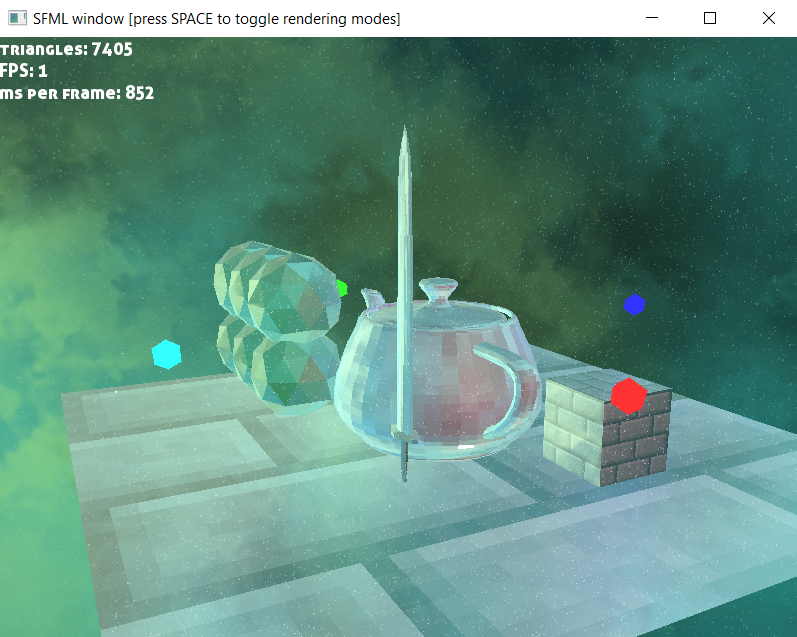
\includegraphics[scale=0.55]{img.png} 
		
\end{frame}
\begin{frame}
	\frametitle{Результаты работы}
	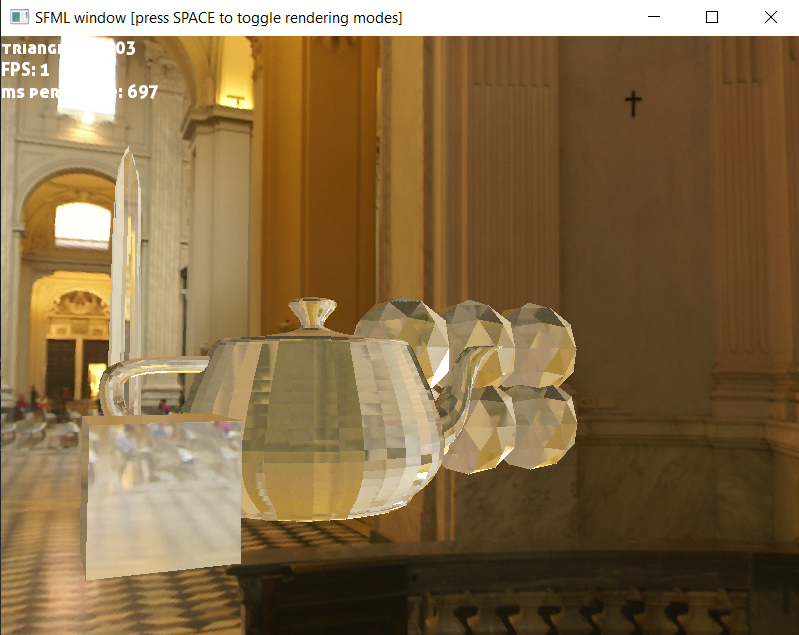
\includegraphics[scale=0.45]{img1.png} 
	
\end{frame}
\begin{frame}
	\frametitle{Результаты работы}
	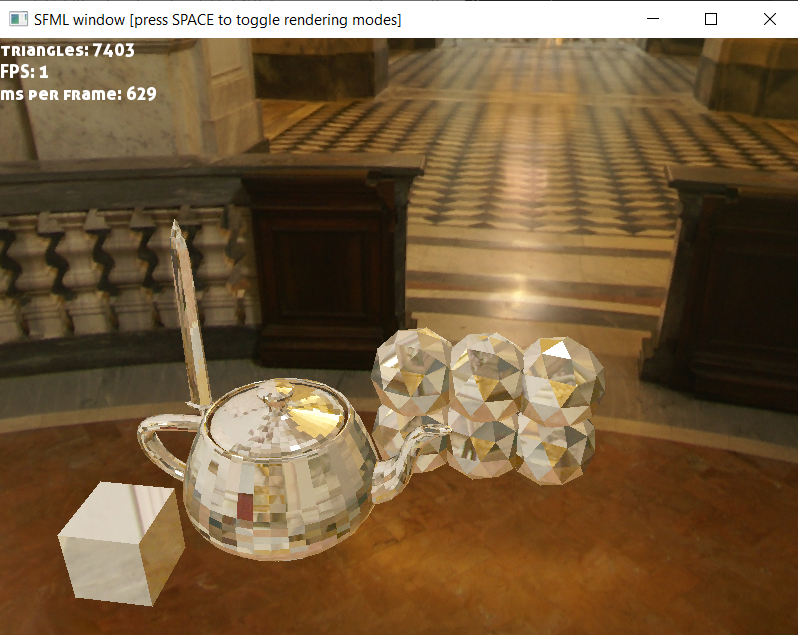
\includegraphics[scale=0.45]{img2.png} 
	
\end{frame}
\begin{frame}
	\frametitle{Результаты работы}
	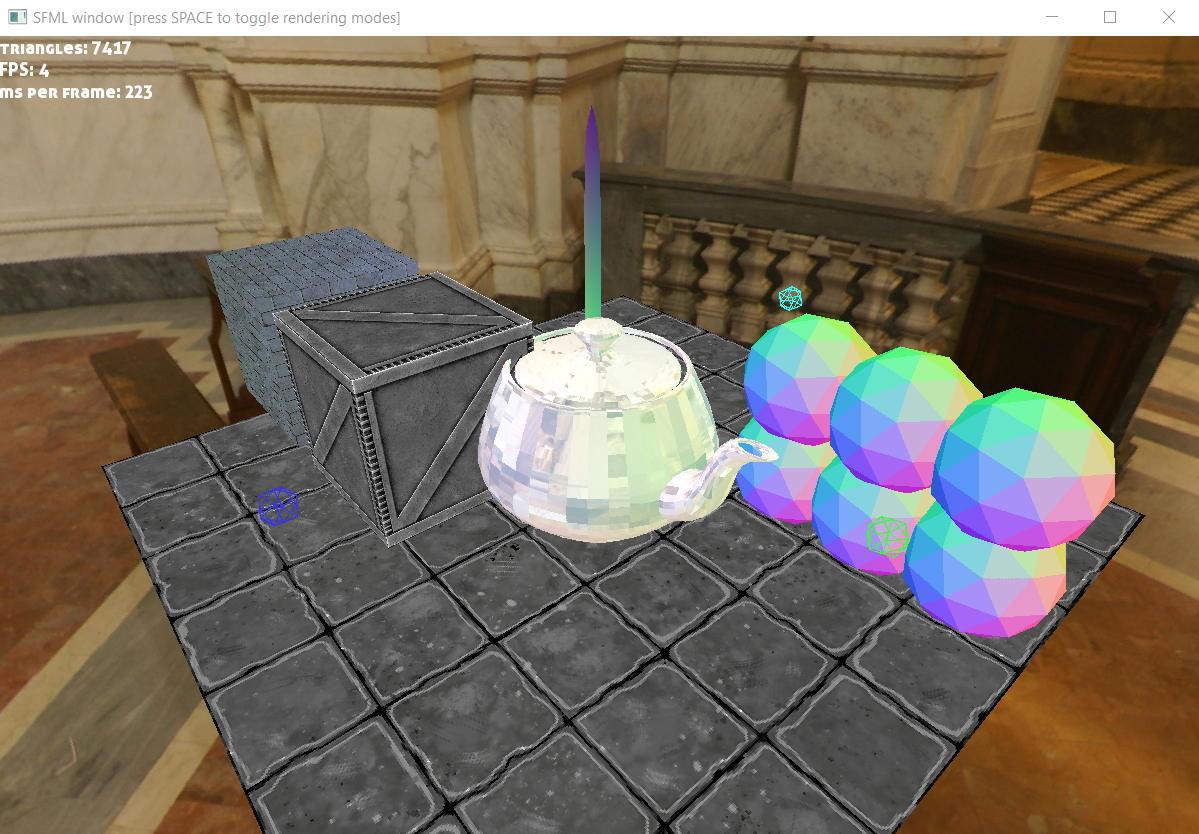
\includegraphics[scale=0.4]{img3.png} 
	
\end{frame}

\begin{frame}
	\frametitle{Результаты работы}
	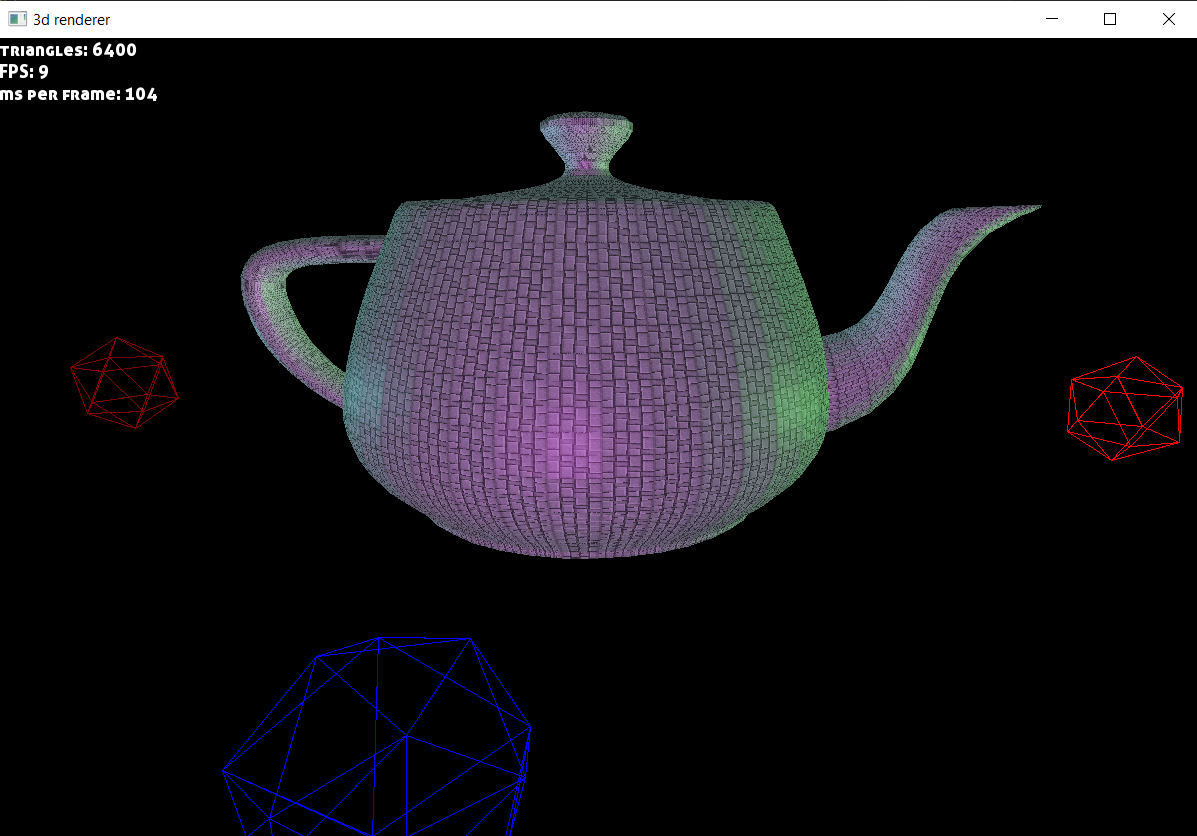
\includegraphics[scale=0.4]{img4.png} 
	
\end{frame}

\begin{frame}
	\frametitle{Результаты работы}
	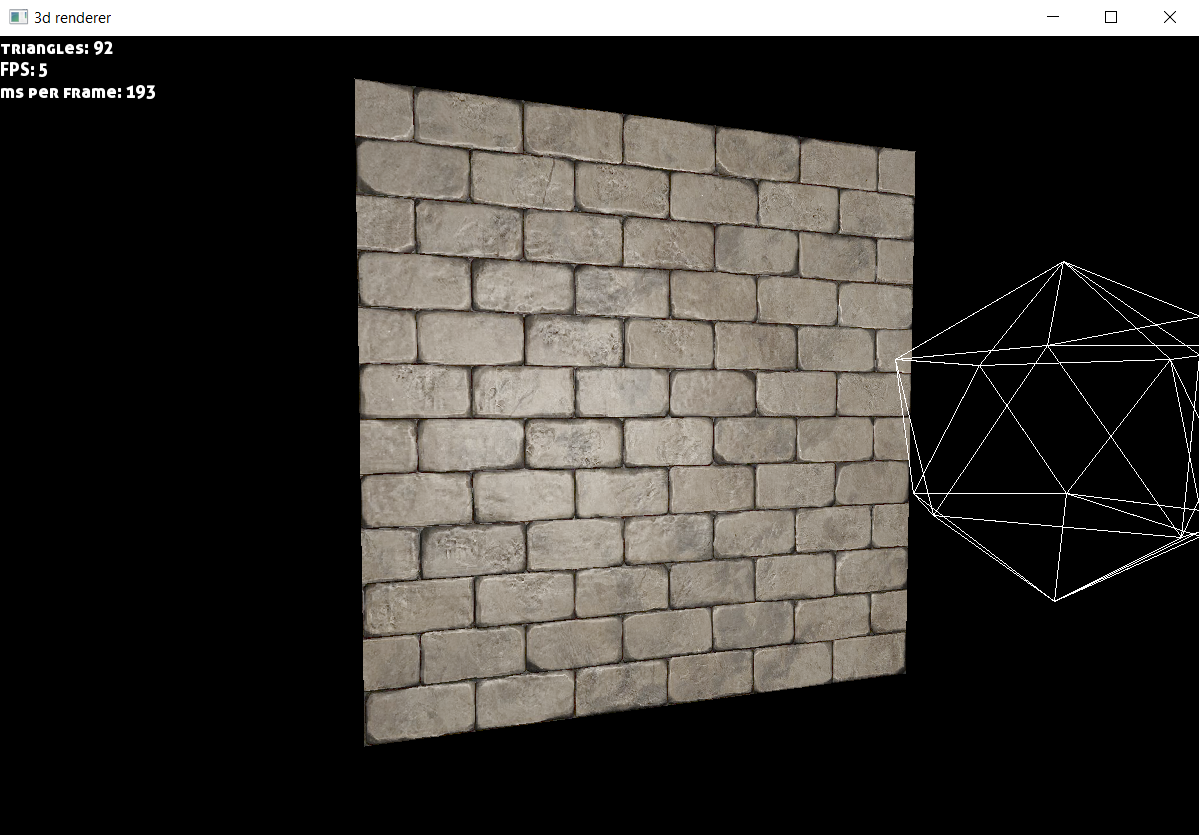
\includegraphics[scale=0.4]{img5.png} 
	
\end{frame}
	
	\begin{frame}
		Спасибо за внимание. 
		
	\end{frame}
	
\end{document}